\chapter{Influence Diagrams}
\label{ch-inf-dia}

This chapter is based on Ref.\cite{sha-inf-dia}.


\begin{figure}[h!]
\centering
\includegraphics[width=3.2in]
{inf-dia/inf-dia-jensen.jpg}
\caption{View of Mount Vesuvius from
  Pompeii}
\label{fig-jensen-diag}
\end{figure}

\begin{figure}[h!]
\centering
\includegraphics[width=6in]
{inf-dia/inf-dia-stages.jpg}
\caption{View of Mount Vesuvius from
  Pompeii}
\label{fig-jensen-stages}
\end{figure}

























Influence diagrams are
just arbitrary bnets
enhanced with a 
new kind of node called an utility node.
The rest
of this brief chapter  will 
be devoted to discussing utility nodes.

Suppose $U(x)$ is a deterministic 
function $U:S_\rvx\rarrow \RR$
called the {\bf utility function}.
Then the {\bf expected utility}
is defined as


\beqa
E_\rvU[\rvU]&=&\sum_UP(U)U
\\
&=&\sum_x\sum_U
\underbrace{P(U|x)}_
{\delta[U, U(x)]}P(x)U
\\
&=&
\sum_xP(x)U(x)
\;.
\eeqa

An {\bf utility node}
can be
understood
as a node
composed of 3 simpler bnet nodes.
This
is illustrated in Fig.\ref{fig-util-node}.

\begin{figure}[h!]
\centering
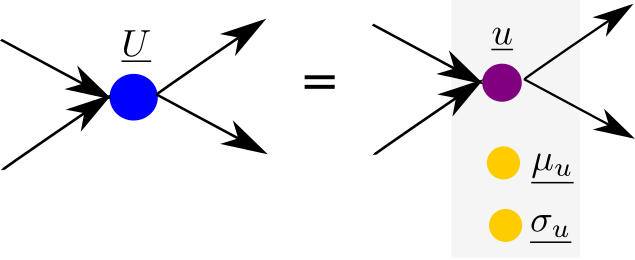
\includegraphics[width=3.5in]
{inf-dia/util-node.png}
\caption{An utility node
can be
understood
as a node 
composed of 3 simpler bnet nodes.} 
\label{fig-util-node}
\end{figure}

The TPMs,
printed in blue,
for the bnet Fig.\ref{fig-util-node},
are as follows:

\beq\color{blue}
P(U|pa(U))=\delta[U, U(pa(U))]
\;,
\eeq
where if $U:S_\rvx\rarrow \RR$,
then $\rvx=pa(\rvU)$.

\beq\color{blue}
P(u|pa(U))=
\delta[u, U(pa(U))]
\eeq

Node $\ul{\mu}_u$
calculates the
expected value (mean value) of $\rvu$:

\beq\color{blue}
P(\mu_u)=\delta(\mu_u,
E_{\rvu}[\rvu])
\eeq

Node $\ul{\sigma}_u$
calculates the
standard deviation of $\rvu$:
\beq\color{blue}
P(\sigma_u)=\delta(\sigma_U,
\sqrt{
E_{\rvu}[
(\rvu-E_{\rvu}[\rvu])^2]})
\eeq

Note that in order to
calculate expected values,
it is necessary that
$\rvU, \rvu\in \RR$. Note that
nodes $\rvu$, $\ul{\mu}_u$, $\ul{\sigma}_u$
must all 3 have access
to the 
TPM
$P(U|pa(U))$ of node $\rvU$.
In fact, in order  to
calculate $E_\rvu[\cdot]$,
it is necessary for
nodes $\ul{\mu}_u$ and 
 $\ul{\sigma}_u$
to have access not just to 
$P(U|pa(U))$ but also to
$P(pa(U))$.

See Fig.\ref{fig-util-merge}.
An influence
diagram may have multiple
utility nodes ($\rvU_1$ and
$\rvU_2$ in Fig.\ref{fig-util-merge}).
Then one can define a merging
utility node $\rvU$ that sums
the values of
all the other utility 
nodes.

\begin{figure}[h!]
\centering
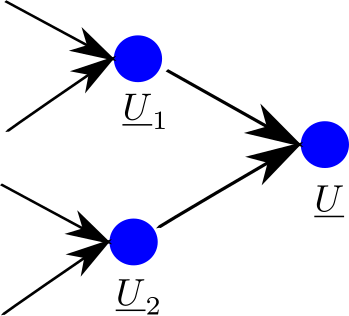
\includegraphics[width=1.5in]
{inf-dia/util-merge.png}
\caption{An influence
diagram may have multiple
utility nodes, say $\rvU_1$ and
$\rvU_2$. Then
one can define an
utility node $\rvU=\rvU_1 + \rvU_2$. } 
\label{fig-util-merge}
\end{figure}

For the node $\rvU$ of 
Fig.\ref{fig-util-merge},
\beq\color{blue}
P(U|U_1, U_2)=\delta(U,U_1 + U_2)
\eeq